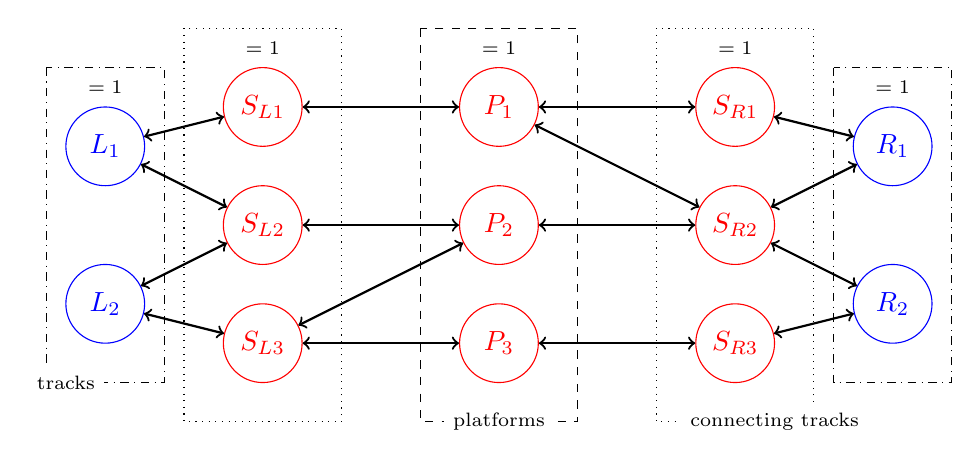
\begin{tikzpicture}
	\tikzstyle{vertex}=[circle,draw,inner sep=0pt, minimum size=1cm]
	
	\node[vertex,blue] at (-5,1) (l1) {$L_1$};
	\node[vertex,blue] at (-5,-1) (l2) {$L_2$};
	
	\node[vertex,red] at (-3,1.5) (sl1) {$S_{L1}$};
	\node[vertex,red] at (-3,0) (sl2) {$S_{L2}$};
	\node[vertex,red] at (-3,-1.5) (sl3) {$S_{L3}$};
	
	\node[vertex,red] at (0,1.5) (p1) {$P_1$};
	\node[vertex,red] at (0,0) (p2) {$P_2$};
	\node[vertex,red] at (0,-1.5) (p3) {$P_3$};
	
	\node[vertex,red] at (3,1.5) (sr1) {$S_{R1}$};
	\node[vertex,red] at (3,0) (sr2) {$S_{R2}$};
	\node[vertex,red] at (3,-1.5) (sr3) {$S_{R3}$};
	
	\node[vertex,blue] at (5,1) (r1) {$R_1$};
	\node[vertex,blue] at (5,-1) (r2) {$R_2$};
	
	\draw[<->,thick] (l1) -- (sl1);
	\draw[<->,thick] (l1) -- (sl2);
	\draw[<->,thick] (l2) -- (sl2);
	\draw[<->,thick] (l2) -- (sl3);
	
	\draw[<->,thick] (sl1) -- (p1);
	\draw[<->,thick] (sl2) -- (p2);
	\draw[<->,thick] (sl3) -- (p2);
	\draw[<->,thick] (sl3) -- (p3);
	
	\draw[<->,thick] (p1) -- (sr1);
	\draw[<->,thick] (p1) -- (sr2);
	\draw[<->,thick] (p2) -- (sr2);
	\draw[<->,thick] (p3) -- (sr3);
	
	\draw[<->,thick] (sr1) -- (r1);
	\draw[<->,thick] (sr2) -- (r1);
	\draw[<->,thick] (sr2) -- (r2);
	\draw[<->,thick] (sr3) -- (r2);
	
	\draw[dashed] (-1,2.5) rectangle (1,-2.5);
	\node[fill=white] at (0,-2.5) {\scriptsize platforms};
	
	\draw[dotted] (-4,2.5) rectangle (-2,-2.5);
	\draw[dotted] (2,2.5) rectangle (4,-2.5);
	\node[fill=white] at (3.5,-2.5) {\scriptsize connecting tracks};
	
	\draw[dashdotted] (-5.75,2) rectangle (-4.25,-2);
	\draw[dashdotted] (4.25,2) rectangle (5.75,-2);
	\node[fill=white] at (-5.5,-2) {\scriptsize tracks};
	
	\node at (-5,1.75) {\scriptsize$\hardcapacity=1$};
	\node at (-3,2.25) {\scriptsize$\hardcapacity=1$};
	\node at (0,2.25) {\scriptsize$\hardcapacity=1$};
	\node at (3,2.25) {\scriptsize$\hardcapacity=1$};
	\node at (5,1.75) {\scriptsize$\hardcapacity=1$};
\end{tikzpicture}